\section{CRUD, Express et MongoDB}
\paragraph{CRUD}C'est un acronym pour \textbf{CREATE}, \textbf{READ}, \textbf{UPDATE} et \textbf{DELETE} dans certaines denomition il existe un dernier element \textbf{EXECUTE}. C'est une liste d'operation que l'on demande au serveur d'executer au travers des requêtes \textbf{POST}, \textbf{GET}, \textbf{PUT} et \textbf{DELETE} respectivement.
\begin{center}
	\makebox[\textwidth]{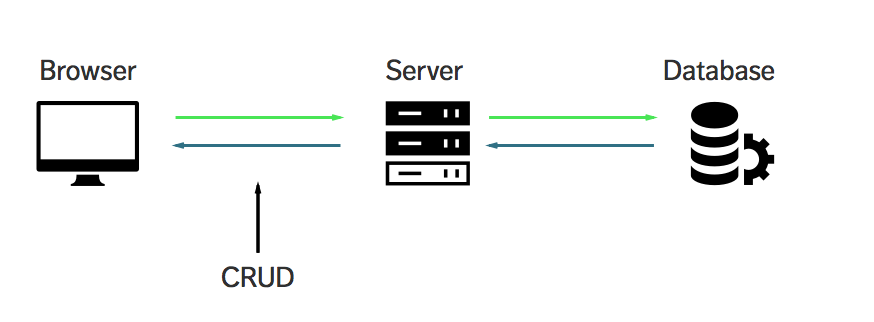
\includegraphics[width=\textwidth]{./media/crud-express-mongo.png}}
\end{center}
\subsection{Middleware}
Nous avons mis dans une classe apart le pilote qui permet de gerer la connection à la base de donnée. On pourra ainsi mettre d'autres pilotes si besoin en supplément de celui qu'on utilise en cas d'evolution ou de partage de donnée.
\lstinputlisting[style=htmlcssjs, firstline=11, lastline=13]{../server/src/tools/db_logic.js}
Chaque invocation de cette fontion permettra d'ouvrir une liaison à la base de donnée.
\subsection{Mongo CRUD}
Nous prendrons juste quelques fonctions comme exemple. En effet il existe une grande variété de fonctions disponibles. Nous avons créer une classe qui génére les requêtes que nous effectuerons. Cette classe n'est toutes fois pas exhaustive. Cela n'empêche que nous avons pris soins de mettre des représentants de chaque type de requetes (les variantes les plus employé, les fonctions qui permettent d'exploiter au mieux la structure de la base de donnée).
Chaque fonction de cette classe fait appel au \textit{driver} que nous avons créé précédement.
Create (création d'une collection)
\lstinputlisting[style=htmlcssjs, firstline=13, lastline=23]{../server/src/tools/crud.js}
Read (selection de tous les elements d'une collection)
\lstinputlisting[style=htmlcssjs, firstline=41, lastline=51]{../server/src/tools/crud.js}
Update (mis à jours de champs de données)
\lstinputlisting[style=htmlcssjs, firstline=81, lastline=93]{../server/src/tools/crud.js}
Delete (suppréssion d'un document)
\lstinputlisting[style=htmlcssjs, firstline=113, lastline=123]{../server/src/tools/crud.js}